\documentclass[pdflatex,sn-mathphys-ay,lineno]{sn-jnl}
\usepackage{graphicx}
\usepackage{amsmath,amssymb,amsfonts}
\usepackage{booktabs}
\raggedbottom
\begin{document}
\title[Within-Family Gains vs External Skill in Fractional SEIT Tuberculosis Forecasts]{Within-Family Gains vs External Skill in Fractional SEIT Tuberculosis Forecasts}
\author[1]{\fnm{Amaury} \sur{de Souza}}\email{amaury.souza@ufms.br}
\author*[2]{\fnm{Francisco Federico} \sur{Garc\'ia Crespi}}\email{fedeg@umh.es}
\affil[1]{\orgdiv{Instituto de F\'isica}, \orgname{Universidade Federal de Mato Grosso do Sul}, \orgaddress{\city{Campo Grande}, \state{Mato Grosso do Sul}, \country{Brazil}}}
\affil[2]{\orgdiv{Department of Computer Engineering}, \orgname{Universidad Miguel Hern\'andez de Elche}, \orgaddress{\city{Elche}, \state{Alicante}, \country{Spain}}}
\abstract{An improvement over an integer-order epidemic model does not necessarily imply useful forecasts. We investigated this distinction by independently reimplementing a fractional-order susceptible--exposed--infectious--treated (SEIT) tuberculosis model using 264 monthly notifications from Brazil (2001--2022). Its integer-order counterpart was refitted independently under the same calibration conditions. We then compared both models with persistence, seasonal naive, and seasonal autoregressive integrated moving average (SARIMA) forecasts across 13 expanding-window origins and leads of 1--12 months. Fractional SEIT achieved lower observed root mean squared error (RMSE) and mean absolute error than integer SEIT at every lead (RMSE at lead 1: 792 versus 1186 cases per month). Yet persistence (390) and SARIMA (536) had lower errors throughout, and the fractional model improved on seasonal naive (1091) only at leads 1--5. The fractional order and the progression rate lay at their lower search bounds; in a single-run sensitivity analysis, lowering the bounds moved both estimates and narrowed the within-family margin without changing its sign. Transmission, removal, and excess-mortality rates varied substantially among near-equivalent fits, although their predicted trajectories were similar. The basic reproduction number and disease-free equilibrium were evaluated only for an autonomous reference, not as properties of the time-varying forecasting system. For this national series, with dependent forecast errors and no formal significance tests, the within-family improvement did not establish competitive forecasting performance against persistence or SARIMA.}
\keywords{Mathematical epidemiology, Fractional-order differential equations, Practical identifiability, Forecast evaluation, Basic reproduction number, Tuberculosis}
\maketitle
\noindent\textbf{ORCID identifiers:} Amaury de Souza (\url{https://orcid.org/0000-0001-8168-1482}); Francisco Federico Garc\'ia Crespi (\url{https://orcid.org/0000-0002-7129-7791}).\par\smallskip
\section{Introduction}
A mechanistic model may closely reproduce tuberculosis notifications yet offer little advantage when forecasting future counts. Compartmental models describe transmission and disease progression through linked states, but their predictions also depend on how those states are mapped to reported cases. Forecasting performance therefore needs to be evaluated on observations excluded from model fitting. Out-of-sample evaluation against simple benchmark forecasts is standard in forecasting practice \citep{tashman2000,hyndman2006,petropoulos2022} and has been applied to epidemic forecasts in evaluations that included null, baseline or naive models \citep{funk2019,reich2019,cramer2022}. For example, a comparison of susceptible--infected--recovered (SIR) and seasonal autoregressive integrated moving average (SARIMA) models for tuberculosis in Kazakhstan found lower forecasting errors with SARIMA \citep{kalizhanova2024}.

Fractional-order models change the temporal structure of compartmental dynamics by replacing ordinary derivatives with operators that depend on the past trajectory. Fractional-order versions of compartmental epidemic models have been fitted to outbreak data, for example a fractional SEIR model for Ebola compared with its classical counterpart \citep{area2015}. Work on integer- and fractional-order epidemiological models has also examined identifiability and predictability using physics-informed neural networks \citep{kharazmi2021}. These studies motivate careful evaluation of fractional formulations, but neither a history-dependent mathematical operator nor improved fit is evidence, on its own, for a biological memory mechanism in tuberculosis.

A lower error than integer SEIT has a different meaning from a lower error than a simple forecast. We distinguish these comparisons by refitting the integer model independently, rather than retaining parameters estimated for the fractional formulation, and then evaluating both models against methods outside the mechanistic family. A favorable within-family result need not imply competitive forecasting.

We applied both comparisons to a fractional-order susceptible--exposed--infectious--treated (SEIT) tuberculosis model using monthly notification counts for Brazil. The fractional and integer formulations were independently fitted with a common observation operator, objective function, kinetic bounds, and initialization procedure. Forecast errors were assessed over expanding-window rolling origins against persistence, seasonal naive, and SARIMA on matched origin--target pairs. A separate, fixed-origin open-loop validation provided a longer-horizon comparison within the SEIT family. The study therefore tests whether a gain within the mechanistic family carries over to forecasting skill against methods outside it; it does not propose a new model.

Mechanistic interpretation raises a related but secondary question: how much can be inferred from estimated epidemic rates? Practical identifiability is commonly examined with profile-based approaches \citep{raue2009,wieland2021}, and parameter uncertainty, identifiability and forecasting in epidemic models are discussed in a primer by \citet{chowell2017}. The relation between parameter identifiability and prediction uncertainty has been examined in a likelihood-based workflow by \citet{simpson2024}. We examine both across a finite set of cost-based fits, while evaluating the basic reproduction number ($R_0$) and disease-free equilibrium (DFE) only for an autonomous reference. These diagnostics qualify interpretation of the model; the external forecast comparison remains the primary analysis.

\section{Methods}

\subsection{Study design and independent-reimplementation scope}

We independently reimplemented the fractional-order SEIT model described in the materials of the original study, which were provided by the collaborating author (a copy of the working manuscript is archived with the code), using monthly tuberculosis notifications for Brazil. The original numerical scripts and complete computational configuration were unavailable. We therefore specified the model, estimation procedure, and forecast evaluation directly, with an independently refitted integer-order SEIT as the within-family comparator. We compared the fitted models against external forecasting benchmarks and examined the stability of derived mechanistic quantities when individual rates were weakly identifiable.



Optimal-control interventions were not evaluated in this study.

\subsection{Data and observation mapping}

The study used 264 consecutive monthly tuberculosis notification counts for Brazil, covering January 2001 to December 2022, supplied by the collaborating data provider. That provider identified DATASUS/SINAN as the general source and described geographic and temporal filtering followed by monthly aggregation. The original query settings could not be recovered. Four documented attempts to reconstruct the series from DATASUS/SINAN did not match the supplied values exactly. There were no missing observations or duplicate months.

The dataset is partitioned into two distinct periods:

\begin{itemize}
\item \textbf{Calibration window}: January 2001 to December 2020 ($N_{\text{cal}} = 240$ months).
\item \textbf{Validation window}: January 2021 to December 2022 ($N_{\text{val}} = 24$ months).
\end{itemize}

Population denominators for 2001--2020 were taken from the 2013 revision of the Brazilian national population projection \citep{ibge2013}. This revision was retained because it reproduces the denominator series supplied with the dataset and covers the whole calibration interval. Later revisions of the projection exist; they were not used, because changing the denominator alters a model input, and the sensitivity of the results to that choice was not assessed. The annual projected total was held constant across the twelve months of each year to form the monthly input grid, which the solver then interpolates linearly to obtain a continuous $N(t)$. This population series covers the complete calibration period. For out-of-sample simulation, population values beyond each training endpoint were generated using a log-linear trend fitted exclusively to population observations available within the corresponding training window:

\[
\begin{aligned}
\ln N(t)&=a_0+a_1t, &&t\le t_{\mathrm{train}}\quad\text{(fitting)},\\
\widehat N(t)&=\exp(\widehat a_0+\widehat a_1t), &&t>t_{\mathrm{train}}\quad\text{(extrapolation)}.
\end{aligned}
\]

No population observations beyond the relevant training endpoint were used.

The observed monthly counts are mapped to the exposed-to-infectious transition flow, rather than to the infectious stock $I(t)$. The predicted count for month $k$ is

\[
\widehat y_k=\int_{t_k}^{t_{k+1}}\sigma E(t)\,dt,\qquad t_{k+1}-t_k=1\text{ month}.
\]

The integral is evaluated by composite ordinary trapezoidal quadrature on the corrected exposed-state values produced by the fractional solver:

\[
\widehat y_k\approx\sum_{j=0}^{m-1}\frac{\delta t}{2}\,\sigma\bigl[E(t_k+j\delta t)+E(t_k+(j+1)\delta t)\bigr],\qquad m\delta t=1\text{ month}.
\]

An auxiliary Caputo accumulator driven by $\sigma E$ does not feed back into the epidemiological states. We did not use its increments as observations: monthly predicted counts were calculated by ordinary integration of the numerical solution for $E(t)$. At $\alpha=1$, the continuous-time accumulator increment equals the corresponding ordinary integral, although discrete approximations may differ slightly.

The model contains no separate detection or notification process. The predicted count is the ordinary integral of the exposed-to-infectious flow, so delays in diagnosis and notification, under-notification and changes in case finding are not represented. The initialization $E(0)=y_0/\sigma$ (below) sets the first monthly count equal to the instantaneous flow $\sigma E(0)$; this is an approximation, because the count is an integral over a month and the system need not be at that flow at $t=0$.

\subsection{Fractional SEIT formulation}

The epidemiological states are susceptible $S$, exposed $E$, infectious $I$, and treated/removed $T$. For $0<\alpha<1$, the Caputo derivative with base point zero is

\[
{}^C D_t^\alpha X(t)=\frac{1}{\Gamma(1-\alpha)}\int_0^t(t-s)^{-\alpha}X'(s)\,ds;
\]

at $\alpha=1$ it reduces to the ordinary derivative. With per-month kinetic rates and reference timescale $\tau_0=1\text{ month}$, the dimensionally consistent equations are

\[
\begin{aligned}
{}^C D_t^\alpha S &=\tau_0^{1-\alpha}\left[\Lambda-\frac{\beta SI}{N(t)}-\mu S\right],\\
{}^C D_t^\alpha E &=\tau_0^{1-\alpha}\left[\frac{\beta SI}{N(t)}-(\sigma+\mu)E\right],\\
{}^C D_t^\alpha I &=\tau_0^{1-\alpha}\left[\sigma E-(\gamma+\mu+d)I\right],\\
{}^C D_t^\alpha T &=\tau_0^{1-\alpha}\left[\gamma I-\mu T\right].
\end{aligned}
\]

With time measured in months, the common scaling factor is numerically one. The auxiliary state satisfies ${}^C D_t^\alpha C=\tau_0^{1-\alpha}\sigma E$, with $C(0)=0$, and is not part of the observation mapping.

Here $\beta$ is the transmission coefficient, $\sigma$ the progression rate from exposed to infectious, $\gamma$ the removal rate into the treated compartment, and $d$ the tuberculosis-attributable excess mortality rate. Natural mortality is fixed at $\mu=1/(74\times12)=1/888\text{ month}^{-1}$. For the global calibration, recruitment is $\Lambda=\mu\bar N_{\mathrm{cal}}$; for each rolling origin it is recomputed from that origin's training population. The unchanged search bounds are $\beta\in[0.01,1.00]$, $\sigma\in[0.01,0.50]$, $\gamma\in[0.05,0.30]$, and $d\in[0.0001,0.05]$, in $\text{month}^{-1}$, and $\alpha\in[0.50,1.00]$. These search bounds are imposed estimation restrictions and do not imply precise identification of the individual rates.

The initial states were set analytically from the first observed monthly count $y_0$, with $q_0=y_0/\tau_0$ and $\tau_0=1\text{ month}$:

\[
\begin{aligned}
E(0)&=\frac{q_0}{\sigma}=\frac{y_0}{\sigma\tau_0}, &
I(0)&=\frac{\sigma E(0)}{\gamma+\mu+d}=\frac{y_0}{(\gamma+\mu+d)\tau_0},\\
T(0)&=0, & S(0)&=N(t_0)-E(0)-I(0).
\end{aligned}
\]

This initialization is a modeling convention rather than a consequence of the monthly observation operator. Initial states were recalculated for each candidate parameter vector, with no additional free parameters. Population $N(t)$ remained an exogenous input.

\subsection{Numerical solution and calibration}

The Caputo initial-value problem was solved with the Diethelm--Ford--Freed predictor-corrector method \citep{diethelm2002}, using the Adams--Bashforth--Moulton predict--evaluate--correct--evaluate (PECE) scheme. The numerical time step was $\delta t=1\text{ month}$; forecasting lead $h$ is defined separately. Numerical resolution was evaluated at $\delta t=1,0.5,0.25$ months while holding fitted parameters fixed. The prespecified numerical checks required monthly relative differences and changes in root mean squared error (RMSE) and mean absolute error (MAE) no greater than 1\%, bias changes no greater than 1\% of the observed mean, and decreasing discrepancies with refinement. These checks assess empirical numerical consistency, not an analytic error bound.

The fractional model estimated $\theta=(\beta,\sigma,\gamma,d,\alpha)$ on January 2001--December 2020 by differential evolution (DE) \citep{storn1997}, with \texttt{best1bin}, \texttt{popsize=15}, \texttt{mutation=(0.5,1.0)}, \texttt{recombination=0.7}, \texttt{tol=0.01}, \texttt{maxiter=1000}, and \texttt{polish=False}. The same configuration and kinetic bounds were used for the independent integer fit. The objective was

\[
J(\theta)=\sqrt{\frac{1}{240}\sum_{k=1}^{240}\bigl(y_k-\widehat y_k(\theta)\bigr)^2}.
\]

Both global fits used random seed \texttt{20260815}. Validation data from 2021--2022 were excluded from calibration and parameter selection. Invalid numerical candidates were assigned penalty $10^{12}$; failed optimization or an invalid final simulation rendered the fit inadmissible.

The first global fit was used as the reference for subsequent diagnostics. Four additional fits used seeds \texttt{20260816}--\texttt{20260819} to examine sensitivity to optimization initialization. Optimizer convergence does not establish uniqueness or parameter identifiability.

\subsection{Integer-order comparator}

To evaluate the specific contribution of fractional differentiation within the SEIT family, an integer-order counterpart is defined by fixing $\alpha \equiv 1.0$.

The kinetic parameters of the integer model, $\theta_{\text{int}}=(\beta,\sigma,\gamma,d)$, were re-estimated independently using the same DE settings, calibration objective, and parameter bounds. Thus, the comparison is between two fitted models; it does not simply set $\alpha=1.0$ while retaining the fractional model's kinetic parameters.

\subsection{Practical-identifiability analysis}

Practical-identifiability diagnostics compared the reference global fit, four additional fits, and parameter profiles, using the same calibration data, ordinary monthly observation operator, bounds, initialization, and optimization settings. Fits were not selected based on validation errors or mechanistic conclusions.

Profiles for $\beta,\gamma,d$ used seven grid points each: the primary value and offsets of 10\%, 30\%, and 60\% of its distance toward each search bound. The $\alpha$ grid was the union of its corresponding seven points with $[0.50,0.505,0.51,0.52,0.55,0.60,0.65,0.70,0.75,0.80,0.85,0.90,0.95,1.00]$, giving 21 distinct points within $[0.50,1.00]$.

For each $\alpha$, a fixed-parameter cost section held $\beta,\sigma,\gamma,d$ at their primary values. Separately, a reoptimized profile fixed $\alpha$ and re-estimated the other four parameters. Each point in all four reoptimized profiles used seed \texttt{20260815}, the same DE configuration, and the original bounds for its four free dimensions. Analytic initial conditions were recomputed when the relevant kinetic parameters changed. Fixed-parameter evaluations were distinguished from reoptimized profile fits.

The explored set comprised the reference fit, four additional optimizations, and 42 reoptimized profile solutions. Fixed-section evaluations were not included in this pool. Its main practical-equivalence region was

\[
\Theta_{1\%}=\left\{\theta\in\Theta_{\mathrm{explored}}:\ J(\theta)\le1.01J(\theta_{\mathrm{primary}})\right\}.
\]

The threshold was defined relative to the reference global cost, not the lowest cost subsequently found. Parameter and prediction dispersion were summarized over this finite set; the resulting cost-based region is neither a confidence set nor an exhaustive bound on admissible parameters. Validation observations did not determine its membership.

For the main 1\% region, monthly prediction dispersion was summarized over its 32 solutions separately for the 240 calibration months (January 2001--December 2020) and the 24 single-origin open-loop validation months (January 2021--December 2022). At each month, the coefficient of variation (CV) was the population standard deviation of the predicted monthly counts across these solutions divided by the absolute value of their mean, reported as a percentage. Reported ranges are the minimum and maximum monthly CVs within each period. They describe between-solution trajectory dispersion, not error against observations, confidence intervals, or external-baseline forecasting skill.

The diagnostic protocol was documented after the forecasting results became available. Its choices should therefore not be regarded as prospectively specified for the entire study.

\subsection{Basic reproduction number and local stability}

The reproduction-number functional and DFE classification were evaluated under an explicitly autonomous reference, with $S^*=\Lambda/\mu$ and constant $N_{\mathrm{ref}}=S^*$. The physical disease-free state is $(S^*,0,0,0)$. For the infected subsystem $(E,I)$, the next-generation decomposition \citep{vandendriessche2002} in this reference is

\[
\mathcal F=\begin{bmatrix}0&\beta\\0&0\end{bmatrix},\qquad
\mathcal V=\begin{bmatrix}\sigma+\mu&0\\-\sigma&\gamma+\mu+d\end{bmatrix},
\]

and

\[
R_0^{\mathrm{ref}}=\rho(\mathcal F\mathcal V^{-1})=\frac{\beta\sigma}{(\sigma+\mu)(\gamma+\mu+d)},\qquad\mu=1/888.
\]

The common positive factor $\tau_0^{1-\alpha}$ cancels in the next-generation matrix. The formula has no explicit $\alpha$ term for fixed kinetic parameters; its evaluated value can nevertheless change when fitting changes those parameters.

With $a=\sigma+\mu$, $b=\gamma+\mu+d$, and $q=S^*/N$, the four-state DFE Jacobian is

\[
J(q)=\begin{bmatrix}
-\mu&0&-\beta q&0\\
0&-a&\beta q&0\\
0&\sigma&-b&0\\
0&0&\gamma&-\mu
\end{bmatrix}.
\]

In particular, the vector-field derivative $\partial F_T/\partial I=\gamma$ is retained. The auxiliary observation state is excluded because it does not feed back into the epidemiological dynamics. In the autonomous reference $q=1$, the eigenvalues are $-\mu,-\mu$ and

\[
\lambda_{\pm}=\frac{-a-b\pm\sqrt{(a-b)^2+4\beta\sigma}}{2}.
\]

The infected block has negative trace and determinant $ab(1-R_0^{\mathrm{ref}})$. Matignon's condition \citep{matignon1996} for the constant-matrix, common-order Caputo linearization is $|\arg\lambda_i|>\alpha\pi/2$ for every eigenvalue. If $R_0^{\mathrm{ref}}<1$, all four eigenvalues are negative and satisfy this condition for $0<\alpha\le1$; if $R_0^{\mathrm{ref}}>1$, a positive real eigenvalue violates it. The equality case is nonhyperbolic and is not automatically classified as asymptotically stable. The reported local classification is restricted to this autonomous reference.

In the fitted forecasting system, $N(t)$ is exogenous and time varying, so $q(t)$ and $J(q(t))$ vary. The disease-free state still satisfies the infection-free equations, but constant-matrix Matignon arguments do not establish its stability in that nonautonomous system. Pointwise spectra alone do not prove nonautonomous stability, and neither the reproduction-number functional nor the reference equilibrium classification implies disappearance of tuberculosis in Brazil.

\subsection{Long open-loop stress test}

The fitted global fractional and integer models were evaluated from a single origin at December 2020. Each simulation continued from its calibration trajectory through January 2021--December 2022, without state reinitialization, data assimilation, or parameter updating. Population beyond training was extrapolated using the training-only trend. This 24-month open-loop evaluation describes long-horizon prediction from one fitted origin; it is neither a multi-origin external-baseline comparison nor a test of DFE stability.

\subsection{Rolling-origin forecasting evaluation}

The expanding-window evaluation used 13 monthly origins from December 2020 through December 2021 and leads $h=1,\ldots,12$ months. The common support comprised 156 origin--horizon pairs per model, with targets within 2021--2022.

At each origin, training contained only observations dated at or before that origin. The population trend, $\Lambda=\mu\bar N_{\mathrm{train}}$, and analytic initialization were constructed from that training window. Fractional and integer SEIT were independently fitted with the monthly integral observation operator, the stated parameter bounds and DE configuration, and seed \texttt{20260815}: 13 fits per model, 26 in total. The fitted trajectory, including its fractional history, then continued in open loop to all 12 leads. Future target counts were retrieved for scoring after the origin's fits and forecasts were complete.

Unlike the fixed 2001--2020 calibration, later rolling origins included the 2021 observations already available at those dates. Model fitting and population extrapolation used only information available at each origin.

\subsection{External forecasting baselines}

Three external benchmarks were evaluated on exactly the same origin--target pairs as SEIT:

\begin{enumerate}
\item \textbf{Persistence:} $\widehat y_{t+h}=y_t$.
\item \textbf{Seasonal naive, lag 12:} $\widehat y_{t+h}=y_{t+h-12}$; for $1\le h\le12$, the referenced observation is available at the origin.
\item \textbf{SARIMA:} $(0,1,2)(1,1,1)_{12}$, with its order selected by Akaike information criterion (AIC) from 36 candidate specifications on the 2001--2020 period. Coefficients were re-estimated on each origin's expanding training window while maintaining the selected order.
\end{enumerate}

We compared the mechanistic predictions with 468 previously recorded baseline forecasts after checking their origin--target alignment. The baseline methods were not rerun when the mechanistic observation operator was revised. The origin-specific SARIMA coefficients were not stored with the original forecasts. We regenerated the 13 fits with the frozen order and the same estimator options; the regenerated forecasts reproduced the archived ones with a maximum relative error of $9.2\times10^{-9}$, and the coefficients are reported in Appendix~\ref{app:tables} (Table~\ref{tab:sarima}).

\subsection{Forecast metrics, relative skill, and horizon descriptors}

At each lead $h$, RMSE, MAE, and mean bias were evaluated over the 13 origins:

\[
\mathrm{RMSE}(h)=\sqrt{\frac1{13}\sum_{i=1}^{13}(\widehat y_{i,h}-y_{i,h})^2},\qquad
\mathrm{MAE}(h)=\frac1{13}\sum_{i=1}^{13}|\widehat y_{i,h}-y_{i,h}|,
\]

\[
\mathrm{Bias}(h)=\frac1{13}\sum_{i=1}^{13}(\widehat y_{i,h}-y_{i,h}).
\]

We also computed a mean absolute scaled error in the spirit of \citet{hyndman2006}, scaling the absolute error for each origin with the in-sample mean absolute error of the seasonal naive forecast with period 12 on that origin's training window (January 2001 to the origin month), and was averaged over the 13 origins at each lead. We refer to it as MASE. Values below one indicate smaller absolute errors than the in-sample seasonal naive on that window. MAE, mean bias and MASE by lead are given in Appendix~\ref{app:tables}.

For error measure $L\in\{\mathrm{RMSE},\mathrm{MAE}\}$, relative skill was

\[
\mathrm{Skill}_L(M,B,h)=1-\frac{L_M(h)}{L_B(h)}.
\]

Positive skill indicates lower observed error than the specified comparator. The integer SEIT comparison is reported separately from the three external baselines.

$H_{\mathrm{relax}}$ is the last lead with strictly positive skill; $H_{\mathrm{strict}}$ is the length of the consecutive positive-skill sequence beginning at $h=1$. Each is zero when its defining positive sequence is absent. Values are reported by comparator and error measure, without pooling horizons or selecting the most favorable reference. They describe this evaluation support and are not universal predictability limits.

\subsection{Statistical interpretation boundary}

The forecasting comparisons are descriptive sample metrics. Forecast errors across overlapping origins and horizons are dependent; no formal predictive-accuracy or significance tests were performed. Lower observed error within the SEIT family is distinguished from external baseline-relative skill and from statistical or generalizable superiority.

\subsection{Sensitivity to the lower bounds of \texorpdfstring{$\alpha$}{alpha} and \texorpdfstring{$\sigma$}{sigma}}\label{sec:sensmethods}

In the primary fits, $\alpha$ and $\sigma$ lay at their lower search bounds. To examine whether these values reflect the data or the bounds, we repeated the global calibration with wider lower bounds, keeping the calibration window, observation operator, initialization, optimizer settings, seed and the remaining bounds unchanged. Four additional fits were run: fractional with $\alpha\in[0.20,1.00]$ and the original bounds of $\sigma$ (F-a); fractional with the original bounds of $\alpha$ and $\sigma\in[0.001,0.5]$ (F-b); fractional with both bounds widened (F-c); and integer with $\sigma\in[0.001,0.5]$ (I-b). The lower bound of $0.001\text{ month}^{-1}$ for $\sigma$ corresponds to a mean progression time from exposed to infectious of about 83 years; it was chosen to relax the constraint, not as a plausible value. A refit of the original configuration was run first as a control and reproduced the primary fit. A fitted $\alpha$ was considered determined by its bound if it lay within 0.01 of the lower bound, and a fitted $\sigma$ if it lay below 1.1 times its lower bound. These rules and the protocol of the fits were written before the fits were run. Numerical resolution was checked as for the other fits, with steps of 1, 0.5 and 0.25 months. Each configuration was fitted once, so differences between fits mix the effect of the bounds with optimizer variability. The fits were evaluated on the calibration window and on the 2021--2022 open-loop validation only; no rolling-origin forecast was produced with the wider bounds.

\subsection{Transient of the exposed compartment}\label{sec:transmethods}

To relate the fitted trajectories to the reference equilibrium, we simulated the 264 months with the primary parameter vectors of both models, without refitting, using the solver and initialization described above. We recorded the inflow $\beta SI/N$ and the outflow $(\sigma+\mu)E$ of the exposed compartment and their ratio $\rho(t)$. For the integer model, we regressed $\log E(t)$ on $t$ over the calibration months and compared the slope with $-(\sigma+\mu)$, the rate of a compartment without inflow. For the fractional model, the corresponding solution without inflow is $E(t)/E(0)=E_\alpha\bigl(-(\sigma+\mu)t^\alpha\bigr)$, with the Mittag-Leffler function $E_\alpha(z)=\sum_{k\ge0}z^k/\Gamma(\alpha k+1)$, and we compared $E(t)/E(0)$ with it. Before running the simulation we fixed the following conventions: the inflow was called negligible if $\rho\le0.10$ throughout the calibration months, and a trajectory was called consistent with a draining reservoir only if the inflow was negligible and, in addition, the integer-model slope was within 10\% of $-(\sigma+\mu)$ or the maximum relative difference of the fractional model to the Mittag-Leffler solution was at most 10\%. These thresholds are conventions, not theoretical values.

\section{Results}

\subsection{Corrected global fit and single-origin open-loop validation}

Both SEIT formulations were calibrated on the same 2001--2020 observations, with their kinetic parameters estimated independently. The resulting parameter vectors appear in Table~\ref{tab:1}. For the fractional fit, $\alpha=0.502203$ lies near the imposed lower bound of 0.50; the individual kinetic rates should not be interpreted as precisely identified epidemiological quantities. The progression rate $\sigma$ also lies at its lower bound in both fits (0.010004 and 0.010173 against a bound of 0.01), so neither value is interpreted as an estimate. The excess-mortality rate $d$ differs by a factor of about 180 between the models (0.0391 and 0.000213 month$^{-1}$; the latter is close to its lower bound of 0.0001), although both describe the same series with calibration errors of the same order (619 and 776 cases per month). The fractional value corresponds to about 0.47 per year. We did not assess its plausibility against independent estimates of tuberculosis-attributable mortality, and we do not interpret $d$ as such an estimate.

\begin{table}[htbp]
\centering
\small
\caption{Estimated parameters for the fractional and integer SEIT formulations. Kinetic parameters are expressed in month$^{-1}$; $\alpha$ is dimensionless.}
\label{tab:1}
\begin{tabular}{@{}lccccc@{}}
\toprule
Model & $\beta$ & $\sigma$ & $\gamma$ & $d$ & $\alpha$ \\
\midrule
fractional & 0.120038 & 0.010004 & 0.261347 & 0.039100 & 0.502203 \\
integer & 0.061166 & 0.010173 & 0.053249 & 0.000213 & 1.000000 \\
\bottomrule
\end{tabular}
\end{table}

The fractional model achieved a calibration RMSE of 619.319, compared with 776.041 for integer SEIT. The advantage remained in the 24-month fixed-origin validation: fractional RMSE/MAE were 1216.542/1035.207, with bias $-$983.954; integer RMSE/MAE were 1759.542/1588.653, with bias $-$1588.653 (Table~\ref{tab:2}; Fig.~\ref{fig:1}). Both models tended to underpredict in this open-loop period. The comparison involves one forecast origin and does not address performance against external benchmarks.

\begin{table}[htbp]
\centering
\small
\caption{Global calibration and open-loop validation. Bias is predicted minus observed; errors are monthly notification counts. The calibration contains 240 months and validation 24 months.}
\label{tab:2}
\begin{tabular}{@{}llrrr@{}}
\toprule
Model & Window & RMSE & MAE & Bias \\
\midrule
fractional & Calibration & 619.319 & 484.062 & 49.457 \\
fractional & Open-loop validation & 1216.542 & 1035.207 & -983.954 \\
integer & Calibration & 776.041 & 616.146 & 171.227 \\
integer & Open-loop validation & 1759.542 & 1588.653 & -1588.653 \\
\bottomrule
\end{tabular}
\end{table}

The fractional comparison involves independently fitted parameter vectors under the retained ordinary observation operator; it does not isolate the effect of changing the operator or fractional order at a fixed parameter vector.

\begin{figure}[htbp]
\centering
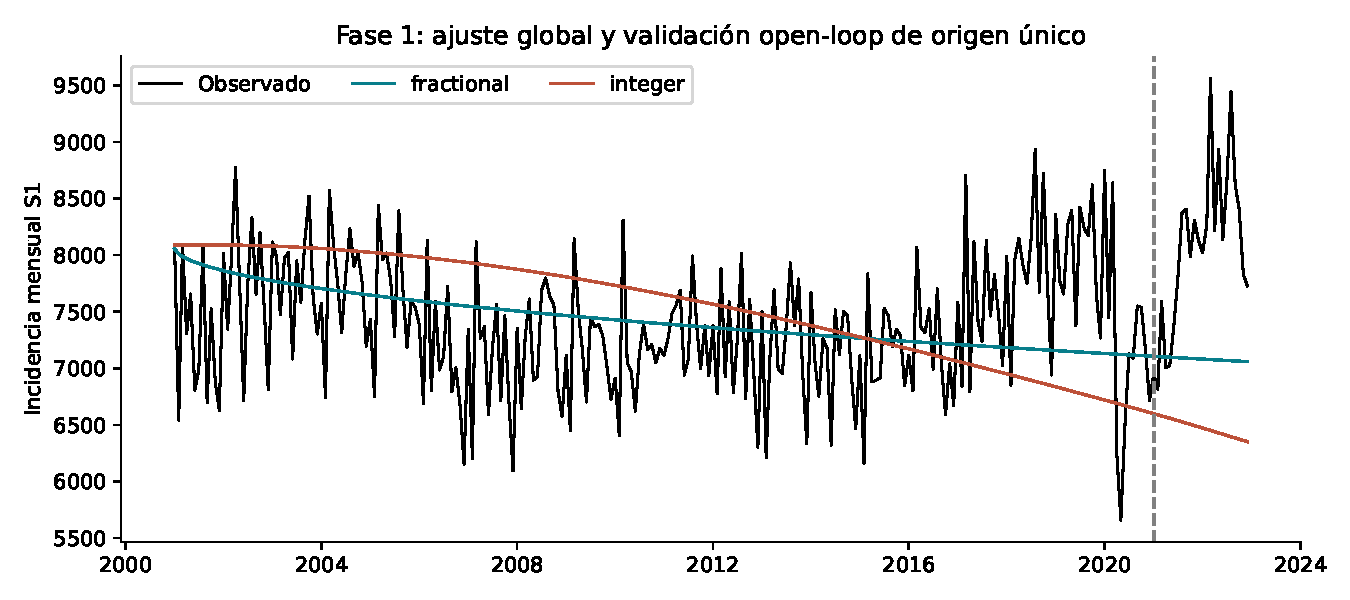
\includegraphics[width=0.96\textwidth]{F1_global_open_loop.pdf}
\caption{Observed monthly counts and the independently fitted fractional and integer SEIT trajectories. The vertical line separates global calibration through 2020 from the fixed-origin open-loop validation. This comparison does not establish external-baseline skill.}
\label{fig:1}
\end{figure}

\subsection{Within-family rolling-origin comparison}

Across all 12 forecast leads, fractional SEIT yielded lower RMSE and MAE than integer SEIT (Table~\ref{tab:3}; Fig.~\ref{fig:2}). Each model contributed 156 forecasts on common origin--horizon pairs, within a total of 780 forecasts from the five methods. All 26 mechanistic fits met their numerical termination criteria. These are observed error differences; no formal test of predictive accuracy was conducted. MAE, mean bias and MASE by lead are given in Appendix~\ref{app:tables} (Tables~\ref{tab:mae_h}--\ref{tab:mase_h}). Persistence and seasonal naive give identical forecasts at $h=12$ in all 13 origins, because both equal the observation at the origin; their errors therefore coincide at that lead (RMSE 1152.958 in Table~\ref{tab:3}). All five methods had negative mean bias, that is, under-prediction, at every lead. MASE was below one only for persistence at $h=1$ and $h=2$ (0.728 and 0.931); at $h=1$ it was 1.491 for fractional SEIT, 2.375 for integer SEIT, 2.347 for seasonal naive and 1.006 for SARIMA.

\begin{table}[htbp]
\centering
\scriptsize
\caption{Rolling-origin RMSE under the common temporal protocol. Each cell summarizes 13 forecasts at one lead. No errors are pooled across leads.}
\label{tab:3}
\begin{tabular}{@{}lrrrrr@{}}
\toprule
Lead (months) & Fractional & Integer & Persistence & Seasonal naive & SARIMA \\
\midrule
1 & 791.588 & 1185.800 & 389.702 & 1090.638 & 535.547 \\
2 & 855.628 & 1281.075 & 494.271 & 1049.835 & 595.827 \\
3 & 1089.172 & 1530.886 & 709.999 & 1170.540 & 725.784 \\
4 & 1127.269 & 1574.968 & 720.287 & 1182.556 & 841.713 \\
5 & 1233.747 & 1710.971 & 832.477 & 1278.390 & 939.654 \\
6 & 1274.003 & 1770.702 & 845.856 & 1239.172 & 1022.421 \\
7 & 1340.440 & 1858.590 & 964.206 & 1237.408 & 1096.024 \\
8 & 1480.861 & 2009.191 & 1077.249 & 1258.413 & 1161.578 \\
9 & 1499.639 & 2037.321 & 1120.357 & 1207.927 & 1213.959 \\
10 & 1501.699 & 2041.686 & 1170.294 & 1189.946 & 1242.805 \\
11 & 1498.888 & 2048.768 & 1175.946 & 1190.754 & 1291.796 \\
12 & 1472.295 & 2022.497 & 1152.958 & 1152.958 & 1283.583 \\
\bottomrule
\end{tabular}
\end{table}

\begin{figure}[htbp]
\centering
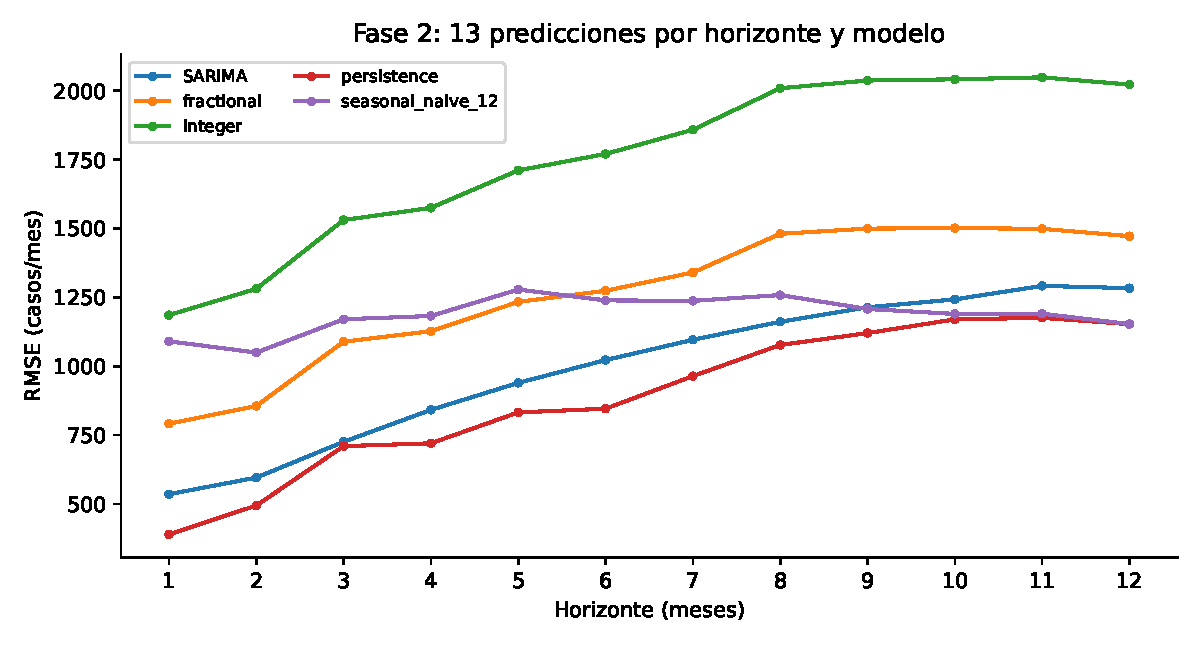
\includegraphics[width=0.96\textwidth]{F2_rolling_RMSE.pdf}
\caption{RMSE at each of the 12 monthly leads for fractional SEIT, integer SEIT, persistence, seasonal naive, and SARIMA, on the same 13-origin support.}
\label{fig:2}
\end{figure}

\subsection{External baseline skill and boundary estimates}

Fractional SEIT did not outperform persistence or SARIMA at any lead. Both benchmarks had lower RMSE and MAE than fractional SEIT at every lead, giving $H_{\mathrm{relax}}=H_{\mathrm{strict}}=0$ for both comparisons. Seasonal naive had higher errors than fractional SEIT at $h=1,\ldots,5$, but lower errors at $h=6,\ldots,12$; both horizon descriptors were therefore 5 (Table~\ref{tab:4}; Fig.~\ref{fig:3}). This five-month window is specific to the seasonal-naive benchmark, not a general limit on tuberculosis predictability.

\begin{table}[htbp]
\centering
\small
\caption{Fractional skill descriptors against four comparators. Positive-lead sets and descriptors are identical for RMSE and MAE; each comparator is reported separately.}
\label{tab:4}
\begin{tabular}{@{}lccc@{}}
\toprule
Comparator & Positive leads & $H_{\mathrm{relax}}$ & $H_{\mathrm{strict}}$ \\
\midrule
Integer SEIT & 1--12 & 12 & 12 \\
Persistence & None & 0 & 0 \\
Seasonal naive & 1--5 & 5 & 5 \\
SARIMA & None & 0 & 0 \\
\bottomrule
\end{tabular}
\end{table}

\begin{figure}[htbp]
\centering
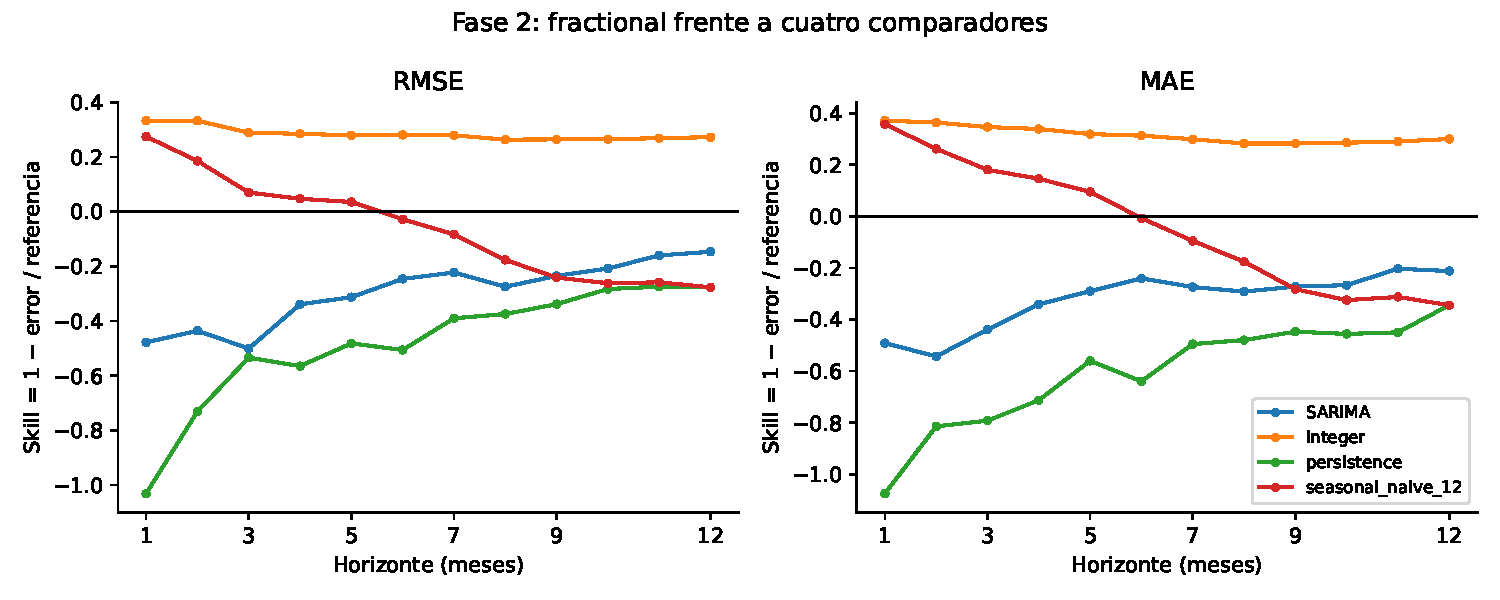
\includegraphics[width=0.96\textwidth]{F3_fractional_skill.pdf}
\caption{Fractional relative skill for (a) RMSE and (b) MAE, separating integer SEIT from the three external benchmarks. The zero line denotes equal error. Positive skill against integer throughout and against seasonal naive only through $h=5$ coexists with negative skill against persistence and SARIMA throughout.}
\label{fig:3}
\end{figure}

Fractional bias was negative at every rolling lead, indicating mean underprediction on this evaluation support.

All 13 fractional fits placed $\alpha$ near the lower search bound, with recorded estimates from 0.500021 to 0.503773. These boundary estimates do not demonstrate epidemiological memory.

\subsection{Secondary diagnostic: fixed and reoptimized alpha profiles}

The reoptimized $\alpha$ profile included points in the main practical-equivalence region from 0.50 to 0.52; the next sampled point, 0.55, was outside it. Figure~\ref{fig:4} contrasts this profile with a fixed-parameter cost section at the same 21 values. Their RMSE values were 618.965 and 618.875 at $\alpha=0.50$, 625.448 and 621.860 at 0.52, and 651.185 and 627.899 at 0.55 (fixed section and reoptimized profile, respectively). The sampled points do not determine a continuous cutoff or establish a unique optimum.

\begin{figure}[htbp]
\centering
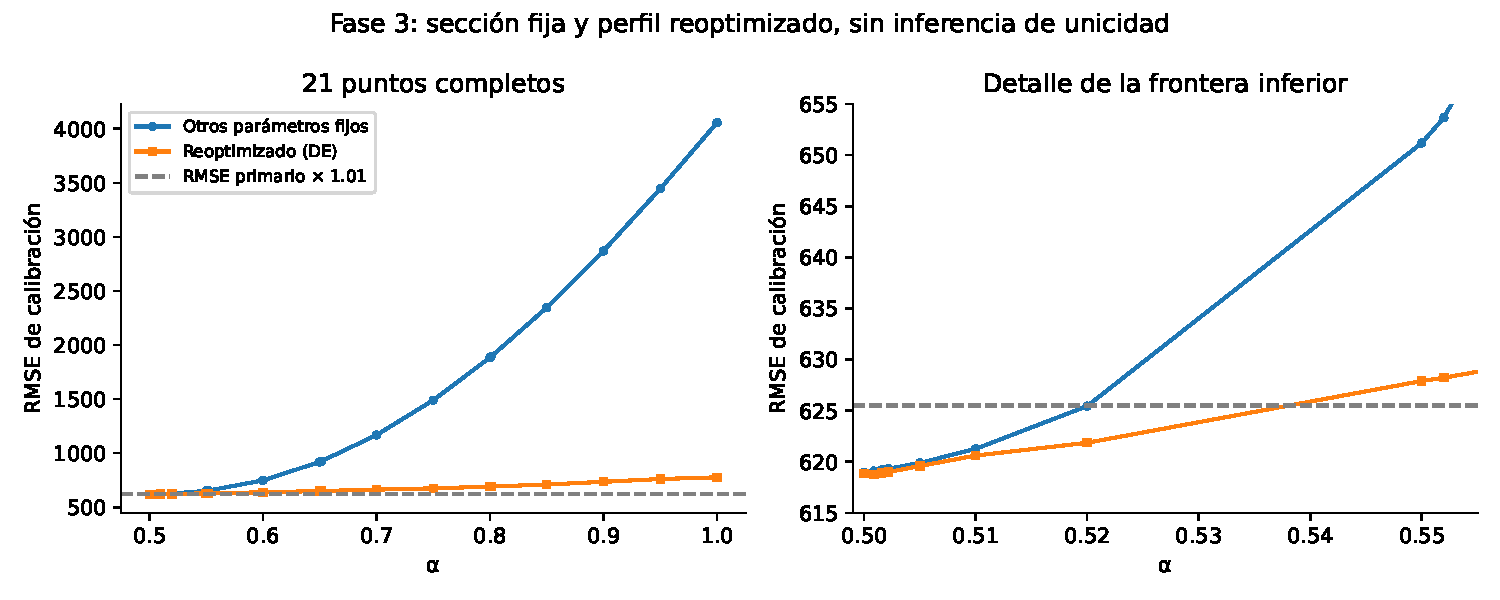
\includegraphics[width=0.96\textwidth]{F4_alpha_profiles.pdf}
\caption{Fixed-section and reoptimized calibration RMSE at (a) all 21 $\alpha$ values and (b) a close view of the lower boundary. The dashed line is the preserved primary RMSE multiplied by 1.01. Connecting lines guide the eye between evaluated points and do not define a continuous confidence region.}
\label{fig:4}
\end{figure}

The 32 fits in the main 1\% practical-equivalence region had markedly different kinetic parameters despite similar calibration errors: $\beta=0.036879$--$0.208034$, $\gamma=0.052711$--$0.297678$, and $d=0.001899$--$0.048114\text{ month}^{-1}$. These ranges indicate limited practical identification within the explored set, rather than precise estimates of the individual rates.

The corresponding monthly prediction coefficients of variation (CVs) were small: 0.0107\%--0.1474\% over the 2001--2020 calibration period and 0.1479\%--0.1595\% over the 2021--2022 fixed-origin validation. Thus, the explored parameter variation produced comparatively similar monthly trajectories. Similarity between predictions, however, is distinct from their errors against observed counts or their skill relative to external benchmarks.

The 1\% threshold, $J\le1.01J(\theta_{\mathrm{primary}})$, was 625.511939 relative to the primary RMSE of 619.318751 (rounded here). The full pool comprised the reference global fit, four additional fits, and 42 reoptimized profiles; 32 solutions met the threshold. This finite, cost-based region was defined relative to the reference fit and is not an exhaustive set of admissible parameters.

\subsection{Secondary diagnostic: reference reproduction number and DFE}

Under the autonomous reference ($\mu=1/888$, $N_{\mathrm{ref}}=S^*=\Lambda/\mu$), the primary value was $R_0^{\mathrm{ref}}=0.357768$. Values for the 32 solutions in the main 1\% region ranged from 0.341657 to 0.587926, all below one. The full pool of 47 solutions spanned 0.341657--1.661998: 44 values were below one and three above (Table~\ref{tab:5}; Fig.~\ref{fig:5}). The three above-one solutions fell outside the main region because of calibration cost. These descriptive ranges are neither confidence intervals nor exhaustive bounds on alternative fits, and they are conditional on the original search bounds (Section~\ref{sec:sens}).

\begin{table}[htbp]
\centering
\scriptsize
\caption{Reference R$_0$ and autonomous DFE classification in the explored sets. The main 32-solution region is a subset of the 47-solution diagnostic pool. Counts and envelopes are descriptive and use the reference defined in Methods.}
\label{tab:5}
\begingroup\setlength{\tabcolsep}{1.8pt}
\begin{tabular}{@{}lrrrrrrr@{}}
\toprule
Explored set & $n$ & $R_0$ min. & $R_0$ max. & $R_0<1$ & $R_0>1$ & Stable DFE & Unstable DFE \\
\midrule
Main 1\% region & 32 & 0.341657 & 0.587926 & 32 & 0 & 32 & 0 \\
Complete diagnostic pool & 47 & 0.341657 & 1.661998 & 44 & 3 & 44 & 3 \\
\bottomrule
\end{tabular}
\endgroup
\end{table}

\begin{figure}[htbp]
\centering
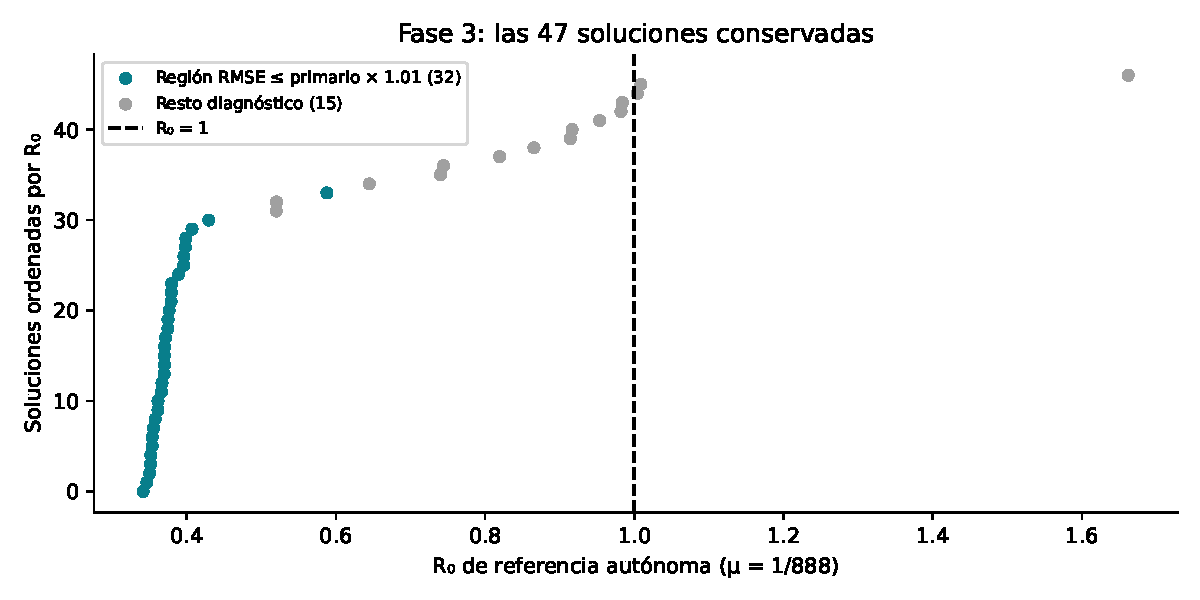
\includegraphics[width=0.96\textwidth]{F5_R0_explored_pool.pdf}
\caption{All 47 reference R$_0$ values, with the 32 solutions admitted by the primary-relative 1\% RMSE criterion distinguished from the remaining diagnostics. The line at one is a reference threshold, not a forecast of disease elimination.}
\label{fig:5}
\end{figure}

Under the autonomous reference, the four-state Jacobian satisfied the common-order Matignon criterion in all 32 admitted solutions, classifying their DFE as locally asymptotically stable. In the complete pool, 44 solutions were classified stable and three unstable, consistent with their reference R$_0$ values. The classification does not establish stability of the fitted system with varying $N(t)$, global stability, or expected disappearance of tuberculosis in Brazil. Pointwise eigenvalue calculations do not constitute a nonautonomous stability proof.

\subsection{Sensitivity to the lower bounds of \texorpdfstring{$\alpha$}{alpha} and \texorpdfstring{$\sigma$}{sigma}}\label{sec:sens}

Table~\ref{tab:sens} shows the additional fits. When the lower bound of $\alpha$ was lowered to 0.20, the fitted $\alpha$ went to the new bound (0.2024 with the original bounds of $\sigma$, 0.2003 with the wider ones), and the training RMSE fell by 4.8--4.9\% (589.3 and 589.2, against 619.3). By the rule defined in Methods, $\alpha$ was determined by its bound in all four fractional fits, so its location is not set by the calibration data in the range examined. When only the bound of $\sigma$ was lowered (F-b), $\alpha$ stayed at 0.5005, $\sigma$ moved to 0.0066 (interior by the rule) and the training RMSE changed by $-0.6\%$, within the 1\% margin used for near-equivalence. With both bounds wider (F-c), $\sigma$ was 0.0359. In the integer model, $\sigma$ went to the new bound (0.0010; training RMSE $-11.2\%$), and $d$ was 0.0093.

\begin{table}[htbp]
\centering
\scriptsize
\caption{Sensitivity of the global fits to the lower bounds of $\alpha$ and $\sigma$. F-0, F-a, F-b and F-c are fractional fits; I-0 and I-b are integer fits (F-0 and I-0 are the primary fits). Ranges are the search bounds; $\hat\alpha$, $\hat\sigma$ and $\hat d$ are the fitted values (month$^{-1}$ for $\sigma$ and $d$). Change is the relative change of the training RMSE against the primary fit of the same model. Valid. RMSE is the open-loop RMSE for 2021--2022. One differential-evolution run per fit (seed 20260815), calibration 2001--2020, ordinary monthly observation operator; bounds of $\beta$, $\gamma$ and $d$ unchanged. No rolling-origin evaluation was run with the wider bounds. $^\dagger$ The maximum pointwise relative change between steps of 1 and 0.25 months was 1.01\% (above the 1\% threshold); changes in RMSE, MAE and bias were below 0.07\%. $^\ddagger$ Computed for this table with the same function as for the fractional fits; not part of the main diagnostics.}
\label{tab:sens}
\begingroup\setlength{\tabcolsep}{2pt}
\begin{tabular}{@{}lllrrrrrrr@{}}
\toprule
Fit & $\alpha$ range & $\sigma$ range & $\hat\alpha$ & $\hat\sigma$ & $\hat d$ & Train RMSE & Change & Valid. RMSE & $R_0^{\mathrm{ref}}$ \\
\midrule
F-0 & 0.5--1 & 0.01--0.5 & 0.5022 & 0.0100 & 0.0391 & 619.3 & -- & 1216.5 & 0.358 \\
F-a$^{\dagger}$ & 0.2--1 & 0.01--0.5 & 0.2024 & 0.0350 & 0.0310 & 589.3 & ($-$4.8\%) & 1086.8 & 0.040 \\
F-b & 0.5--1 & 0.001--0.5 & 0.5005 & 0.0066 & 0.0081 & 615.8 & ($-$0.6\%) & 1195.6 & 0.039 \\
F-c$^{\dagger}$ & 0.2--1 & 0.001--0.5 & 0.2003 & 0.0359 & 0.0309 & 589.2 & ($-$4.9\%) & 1078.6 & 0.070 \\
I-0 & 1 & 0.01--0.5 & 1 & 0.0102 & 0.0002 & 776.0 & -- & 1759.5 & 1.009$^{\ddagger}$ \\
I-b & 1 & 0.001--0.5 & 1 & 0.0010 & 0.0093 & 689.1 & ($-$11.2\%) & 1375.3 & 0.809 \\
\bottomrule
\end{tabular}
\endgroup
\end{table}

The validation RMSE for 2021--2022 was lower in the wider-bound fits: by 1.7\% (F-b) to 11.3\% (F-c) for the fractional model and by 21.8\% for the integer model (I-b). The ordering of the two models did not change: every fractional fit had lower training and validation RMSE than I-b (validation 1078.6--1195.6 against 1375.3). The size of the difference did change. With the same lower bound of $\sigma$ (0.001) for both models, the fractional validation RMSE was 13\% lower than the integer one (F-b against I-b; 1195.6 and 1375.3), against 31\% lower in the primary fits (1216.5 and 1759.5). In training, the corresponding differences were 11\% and 20\%.

The reference $R_0$ was 0.039 (F-b), 0.070 (F-c) and 0.040 (F-a), against 0.358 for the primary fit. All of them are below one, but they lie below the whole range of explored solutions in the main analysis (0.3417--1.6620), although the training RMSE of F-b differs from the primary by only 0.6\%. The reference $R_0$ of the primary integer fit is 1.009 and that of I-b 0.809; these values were not part of the main diagnostics. Two fits (F-a and F-c) slightly exceeded the 1\% threshold for the maximum pointwise change between steps of 1 and 0.25 months (1.01\% in both), while the changes in RMSE, MAE and bias were below 0.07\%. We report them as descriptive fits with this limitation. Each fit is a single optimizer run, and none was evaluated in the rolling-origin comparison.

\subsection{Transient of the exposed compartment}\label{sec:trans}

Under the primary parameters, the exposed compartment declined slowly in both models, from about 0.8 million individuals at $t=0$ ($E(0)=y_0/\sigma$): by 12\% in the fractional and 18\% in the integer model over the 240 calibration months. In neither model was the inflow negligible. In the integer model, the ratio $\rho$ of inflow to outflow decreased from 1.003 to 0.857 over the calibration months, so the inflow replaced between 86\% and 100\% of the outflow; the slope of $\log E$ was $-0.00087\text{ month}^{-1}$, 7.7\% of the pure-decay rate $-(\sigma+\mu)=-0.0113\text{ month}^{-1}$. In the fractional model, $\rho$ ranged from 0.298 to 0.361, and $E(t)/E(0)$ stayed within 5.9\% of the Mittag-Leffler solution without inflow over the calibration months. That agreement is permissive because the total decline is small: at month 240, $E/E(0)$ was 0.879 against 0.830 for the solution without inflow, that is, a decline of 12.1\% against 17.0\%. Neither trajectory therefore met the criterion for a draining reservoir defined in Methods.

\subsection{Numerical and temporal checks}

Numerical-resolution checks satisfied the stated thresholds for 26 rolling-origin and 115 global, profile, and diagnostic evaluations. The largest relative monthly difference in the latter group was approximately 0.119134\%, below the 1\% threshold. Refinement did not change the signs of rolling forecast skill or membership in the main practical-equivalence region. Complete refined-grid state trajectories were not retained for every diagnostic fit.

\section{Discussion}

The two forecast comparisons lead to different conclusions. Fractional SEIT improved on its independently refitted integer-order counterpart, both in the single-origin open-loop evaluation and across the 13 rolling origins. But persistence and SARIMA had lower RMSE and MAE at all twelve rolling leads. The within-family advantage was thus observed on this evaluation support without making the fractional formulation competitive with those external forecasting methods.

Refitting the integer model is important for interpreting the within-family comparison. Both formulations used the same observation operator, training observations, kinetic bounds, initialization rule, and optimization settings; the fractional fit also estimated $\alpha$. Their error difference therefore reflects the fitted formulations as a whole, including the different kinetic parameters. It cannot be attributed solely to changing the derivative order at a fixed parameter vector. Moreover, integer SEIT was less accurate than all three external benchmarks at every lead, so outperforming it alone would have overstated the practical forecasting value of the fractional model.

The size of the within-family advantage also depends on the search bounds. In the sensitivity fits the fractional model kept lower training and validation RMSE than the integer model in every comparison, but the validation difference between F-b and I-b, which share the lower bound of $\sigma$, was 13\% against 31\% in the primary fits. We did not repeat the rolling-origin comparison with the wider bounds, so we cannot say how the lead-by-lead differences or the skill against the external benchmarks would change. The ordering reported for the primary fits is therefore conditional on the original bounds, and the size of the margin should not be read as a property of the fractional operator.

The conclusion also depends on which external forecast serves as reference. Fractional SEIT improved on seasonal naive through $h=5$, but not at longer leads; it never improved on persistence or SARIMA. Mean forecast bias was negative at every rolling lead. Because the 13 origins produce overlapping errors across 156 origin--horizon pairs and only 24 distinct target months, the comparison remains descriptive: no predictive-accuracy tests were performed. These results do not support preferring the fitted fractional SEIT over persistence or SARIMA for the evaluated task.

The evaluation window follows a period in which official reports document a fall and a later recovery of tuberculosis notifications. Globally, the World Health Organization reports 7.1 million people newly diagnosed and notified in 2019 (new and relapse cases), a reduction of 18\% to 5.8 million in 2020, a partial recovery to 6.4 million in 2021, and 7.5 and 8.2 million in 2022 and 2023 \citep{who2024}. For Brazil, the Ministry of Health reports 78,487 new cases in 2019, 69,422 in 2020, 73,121 in 2021, 81,604 in 2022 and 80,012 in 2023 (preliminary) \citep{moh2024}, which correspond to a change of $-11.5\%$ in 2020 and of $+5.3\%$ and $+11.6\%$ in 2021 and 2022. Both sources attribute the fall to COVID-related disruptions of health services, and the Ministry of Health also describes the recovery of 2022 as following two years of pandemic-related interruptions \citep{who2024,moh2024}.

Our series follows the same pattern, but it is not directly comparable with these official counts. The annual mean of the monthly counts moves in the same direction ($-10.2\%$, $+6.2\%$ and $+10.9\%$; 8,015 in 2019, 7,201 in 2020, 7,648 in 2021 and 8,484 in 2022), although its level differs from the official counts of new cases and its original extraction could not be recovered. The attribution to COVID-related disruptions is that of the official sources; this study does not test the cause of the changes in the series.

All five methods under-predicted on average at every lead (Table~\ref{tab:bias_h}). The fitted SEIT trajectories are smooth and cannot represent a rebound of this kind, whereas persistence, and SARIMA through its differencing, adapt to the most recent level. The advantage of these two methods may therefore be specific to this post-disruption support, a possibility we could not test because no origin before 2020 was evaluated.

Earlier work provides useful context but answers different questions. Integer- and fractional-order epidemic models have been examined for identifiability and predictability using physics-informed neural networks \citep{kharazmi2021}, while a tuberculosis study in Kazakhstan found SARIMA to forecast more accurately than SIR \citep{kalizhanova2024}. Neither comparison uses the Brazilian SEIT formulation, observation mapping, and common rolling-origin support evaluated here. Our contribution is the resulting empirical assessment of within-family improvement against methods outside that family, not a claim of historical priority for such comparisons.

The identifiability results limit what can be inferred from the fitted individual rates. Among the 32 solutions whose calibration RMSE was within 1\% of the reference fit, $\beta$ ranged from 0.036879 to 0.208034, $\gamma$ from 0.052711 to 0.297678, and $d$ from 0.001899 to 0.048114 month$^{-1}$. Similar agreement with observed monthly counts thus arose from substantially different parameter vectors. This is evidence of limited practical identification in the explored set, not a structural non-identifiability result.

Predictions from those same solutions varied much less than their individual parameters. Across months, the CV ranged from 0.0107\% to 0.1474\% during calibration and from 0.1479\% to 0.1595\% during fixed-origin validation. These values measure agreement among fitted trajectories, not agreement with observations. In fact, similarly shaped trajectories can share systematic errors: the primary fractional fit underpredicted in the open-loop validation, and its rolling forecasts had negative skill against persistence and SARIMA. In this evaluated set, similarity of trajectories does not by itself establish forecast accuracy.

Numerical refinement addresses a separate concern: whether predictions at a fixed parameter vector change materially with solver resolution. The recorded checks support the numerical consistency of the comparisons but say nothing about unique parameter recovery. Likewise, the 1\% RMSE subset is not a likelihood-based confidence region or predictive interval. Likelihood-based approaches can connect parameter uncertainty with prediction \citep{simpson2024}, but such an interpretation is not warranted for this descriptive cost threshold. The diagnostic protocol was documented retrospectively relative to the forecasting results and is not presented as prospectively specified for the entire study.

The estimated fractional order provides another constraint on interpretation. Its global value was $\alpha=0.502203$, and the rolling estimates clustered near the imposed lower bound of 0.50. The sampled reoptimized profile admitted values between 0.50 and 0.52 under the main criterion, whereas 0.55 fell outside it. This result depends on the evaluated grid and search bounds; it does not identify an interior optimum, a continuous uncertainty interval, or a biological memory mechanism. When the lower bound was lowered to 0.20, the fitted order went to the new bound (Table~\ref{tab:sens}) and the calibration RMSE fell by about 4.9\%, so the location of $\alpha$ is set by the search range rather than by the data. The same holds for $\sigma$ in the integer model, which went to 0.001 when allowed.

Three fitted values call for caution. The progression rate $\sigma$ sat at its lower bound, so that $E(0)=y_0/\sigma$ is about 0.8 million individuals; with $\sigma$ free below 0.01 it moved to 0.0066 in the fractional model (a mean progression time of 12.6 years) and to the new bound of 0.001 in the integer model (83 years). The excess-mortality rate of the fractional fit, $d=0.0391\text{ month}^{-1}$ (about 0.47 per year), is about 180 times that of the integer fit, has not been checked against independent mortality estimates, and fell to 0.031 or 0.0081 in the wider-bound fits. Finally, $\alpha$ lay at its bound in every fractional fit. None of these values is interpreted as an estimate of a biological quantity.

The derived reproduction number was more consistent in threshold classification than in exact value within the main explored region. For the autonomous reference $N_{\mathrm{ref}}=S^*=\Lambda/\mu$, the primary value was $R_0^{\mathrm{ref}}=0.357768$, and all 32 near-equivalent solutions were below one (0.341657--0.587926). Their DFEs satisfied the common-order local stability criterion. This agreement pertains to the specified reference and cost-based subset; it does not imply that $R_0$ is precisely identified. Nor is it independent of the original search bounds: the fits with wider bounds gave reference values of 0.04--0.07 (Table~\ref{tab:sens}).

The larger diagnostic pool shows why the subset matters. Of 47 explored solutions, 44 had $R_0^{\mathrm{ref}}<1$ and a stable reference DFE, while three had $R_0^{\mathrm{ref}}>1$ and an unstable DFE. Those three solutions were not removed because of their stability classification; their calibration costs placed them outside the main 1\% region. The apparently uniform reference conclusion therefore depends on the chosen practical-equivalence criterion.

The reference $R_0<1$ and the stability of the disease-free equilibrium describe the asymptotics of the linearized autonomous system, not the mechanism that generates the fitted trajectory. Over the 240 calibration months the exposed compartment of the primary fits declined only slowly (12\% in the fractional and 18\% in the integer model) from a large initial reservoir fixed by $E(0)=y_0/\sigma$, and the inflow $\beta SI/N$ replaced about 30\% (fractional) or most (integer) of the outflow $(\sigma+\mu)E$. Neither trajectory decays at the rate $\sigma+\mu$ that a compartment without inflow would follow. The fitted notifications are thus produced by a large, slowly changing exposed stock, and a reference $R_0<1$ does not by itself indicate that the series is approaching an infection-free state. For the integer primary fit the reference $R_0$ is about 1.009 (Table~\ref{tab:sens}), just above the threshold, whereas for the fractional primary fit it is 0.358.

The reference calculation cannot establish stability of the fitted forecasting system. Population $N(t)$ varies exogenously in that system, making the linearization depend on time through $S^*/N(t)$. Frozen-time eigenvalues are not a stability proof for the resulting nonautonomous equations. Accordingly, the reference DFE classification should not be interpreted as global stability, disappearance of tuberculosis in Brazil, or evidence of forecast accuracy.

For this model and dataset, independent refitting showed that the fractional formulation improves on integer SEIT, while external benchmarks showed that the improvement is insufficient for competitive forecasting against persistence and SARIMA. The identifiability and reference-equilibrium diagnostics further limit mechanistic interpretation. Evaluating these questions separately makes the evidence easier to interpret without treating a favorable model-family comparison as a forecasting recommendation.

\subsection{Limitations}

The findings are limited to one national series. The monthly case counts come from a file whose original extraction route could not be recovered: a pre-specified audit of four DATASUS/SINAN TabNet configurations did not reproduce the 264 monthly values exactly, and the closest configuration differed in 99 months. We did not repeat the forecasting comparison with any of these alternative reconstructions, so we cannot quantify how sensitive the results are to the provenance of the series.

The two forecast evaluations also answer different questions: later rolling origins incorporate 2021 observations already available at each origin, while the fixed-origin test keeps the 2001--2020 fit unchanged. The evaluation window (2021--2022) follows the disruption of 2020, and we did not evaluate origins before 2020, so we cannot say whether the ordering of the methods holds outside this post-disruption period. The results should be read as specific to the window studied.

All comparisons of forecast accuracy are descriptive. With 13 origins, multi-step errors that overlap across origins and a single evaluation window, tests of equal predictive accuracy, such as the Diebold--Mariano test \citep{diebold1995} with the small-sample correction of Harvey, Leybourne and Newbold \citep{harvey1997}, would have little power and rest on assumptions that the sample cannot check, and no inferential protocol was specified before the evaluation. Statements about which method forecasts better should be read as observations for this series and window, not as evidence of a general difference.

The SEIT models as evaluated have no seasonal component, whereas the seasonal naive and SARIMA baselines use the 12-month cycle explicitly. The comparison therefore mixes differences in model class with differences in how seasonality is represented. A seasonal forcing of the transmission rate, for example $\beta(t)=\beta_0\left(1+\varepsilon\cos(2\pi t/12+\varphi)\right)$, would add two parameters and define a different model; we did not fit it. The positive skill of the fractional model against seasonal naive, limited to the first five leads, should not be read as an advantage of the fractional operator over a seasonal specification.

The sensitivity analysis to the search bounds rests on one optimizer run per configuration, did not include a rolling-origin evaluation, and two of its fits slightly exceeded the numerical-resolution threshold for the maximum pointwise change between time steps (1.01\% against 1\%). The seasonal moving-average coefficient of the SARIMA baseline lies at the invertibility boundary in every origin, so its standard errors are not informative (Appendix Table~\ref{tab:sarima}). Some refined-grid diagnostic trajectories were not retained. These gaps restrict independent reconstruction of parts of the analysis but do not change the observed error comparisons.

\section{Conclusions}

We evaluated a fractional-order SEIT tuberculosis model against an independently refitted integer-order version and three external forecasting benchmarks. In the 13-origin rolling evaluation, fractional SEIT had lower RMSE and MAE than integer SEIT at every lead from $h=1$ to $h=12$. It did not outperform persistence or SARIMA at any lead, and its advantage over seasonal naive ended at $h=5$.

The gain over integer SEIT therefore did not translate into competitive forecasting against the stronger external benchmarks. This conclusion concerns the fitted formulations, calibration restrictions, and single Brazilian monthly series examined here. Forecast errors overlap across origins and horizons, so the observed differences are descriptive rather than evidence of statistical or generalizable superiority.

The fractional order and the progression rate lay at their lower search bounds and moved to the new bound or away from it when the bounds were lowered; with a shared bound on the progression rate, the within-family margin narrowed without changing its sign. The secondary diagnostics showed limited practical identification of individual rates despite relatively similar predicted trajectories among near-equivalent fits. This similarity did not imply forecast accuracy. Reproduction-number and DFE results were confined to an autonomous reference and cannot establish stability of the time-varying forecasting system or tuberculosis elimination in Brazil.

\section{Statements and Declarations}

\subsection{Funding}

No funding was received for this study.

\subsection{Competing Interests}

The authors declare that they have no competing interests.


\subsection{Author Contributions}

Amaury de Souza provided the original SEIT tuberculosis study materials and the Brazilian surveillance dataset, described the data preparation procedures, and contributed to the epidemiological context and scientific framing of the study.

Francisco Federico Garc\'ia Crespi designed and conducted the independent model reimplementation, developed and evaluated the computational methodology, performed model calibration, numerical verification, forecasting comparisons, practical-identifiability and stability analyses, and verified data provenance. He also prepared the revised manuscript.

Both authors contributed to defining the scientific question and discussing the interpretation of the findings.


\subsection{Ethics Approval and Consent to Participate}

This study used exclusively secondary, aggregated monthly tuberculosis notification data for Brazil. No individual-level or personally identifiable information was accessed, and no human participants were recruited or contacted. Therefore, ethics committee approval and informed consent to participate were not required.

\subsection{Consent for Publication}

Not applicable unless the final manuscript includes identifiable individual material, which the present manuscript does not.

\subsection{Data Availability}

The Brazilian monthly tuberculosis notification series (January 2001--December 2022; 264 observations) is accessible through the public project repository at \url{https://github.com/fedeg-umh-es/tb-fractional-seit-brazil} and in the Zenodo deposit (DOI: \url{https://doi.org/10.5281/zenodo.23298329}). The file contains aggregate national counts and no individual-level fields. The data provider identified DATASUS/SINAN as its general source and described aggregation to monthly counts. The exact extraction settings could not be recovered: none of four documented DATASUS/SINAN reconstructions reproduced the supplied series exactly, and the closest differed in 99 of 264 months. Consequently, the original extraction is not independently reproducible. Population denominators were obtained from the 2013 Brazilian population projections issued by IBGE \citep{ibge2013}. The series is released under the Creative Commons Attribution 4.0 International licence (CC BY 4.0), and the code under the MIT licence; this does not change the unrecovered provenance of the series described above.

\subsection{Code Availability}

The code implementing the fractional differential equation solver, the differential evolution calibration, the ordinary monthly observation operator, the practical-identifiability and stability analyses and the rolling-origin benchmarks, together with the numerical results supporting this article, is archived at Zenodo (version DOI: \url{https://doi.org/10.5281/zenodo.23298329}; release \texttt{v1.0.0}) and is publicly available in the GitHub repository \url{https://github.com/fedeg-umh-es/tb-fractional-seit-brazil}. The evidence on which the results are based is the frozen package \nolinkurl{evidence_S1/TB_SEIT_EVIDENCE_FREEZE_2026-10-10/} (branch \nolinkurl{evidence/s1-freeze-2026-10-10}, commit \texttt{53eae1091f652ec03937\allowbreak 07f4e0ae7b2ec4b43acb}, whose integrity can be checked with the verification script included in the package. The additional analyses reported here (sensitivity to the search bounds, transient of the exposed compartment, additional forecast metrics and SARIMA coefficients) are in the folder \texttt{analyses/} of the same release. Results obtained with an earlier observation operator are kept in the repository as historical evidence and are not used in this article. The code is released under the MIT licence and the data, results and documents under CC BY 4.0.

\subsection{AI Assistance Disclosure}

The code was generated using artificial intelligence tools and reviewed by the human authors.

\begin{appendices}
\renewcommand{\theHtable}{A\arabic{table}}

\section{Additional forecast metrics and SARIMA coefficients}\label{app:tables}

Tables~\ref{tab:mae_h}--\ref{tab:mase_h} report mean absolute error, mean bias (predicted minus observed) and mean absolute scaled error by lead for the five methods on the 13-origin rolling-origin support. They are computed from the same 780 forecasts as Table~\ref{tab:3}. Table~\ref{tab:sarima} reports the origin-specific SARIMA coefficients.

\begin{table}[htbp]
\centering
\small
\caption{Mean absolute error (cases per month) by lead and method, rolling origin (13 origins).}
\label{tab:mae_h}
\begingroup\setlength{\tabcolsep}{6pt}
\begin{tabular}{@{}lrrrrr@{}}
\toprule
Lead (months) & Fractional & Integer & Persistence & Seasonal naive & SARIMA \\
\midrule
1 & 661.7 & 1052.2 & 318.9 & 1029.8 & 443.8 \\
2 & 740.4 & 1164.0 & 408.2 & 1002.9 & 479.9 \\
3 & 906.2 & 1386.2 & 505.7 & 1105.8 & 629.8 \\
4 & 955.2 & 1444.8 & 557.8 & 1118.4 & 712.3 \\
5 & 1091.9 & 1603.8 & 699.9 & 1206.6 & 846.7 \\
6 & 1168.0 & 1700.2 & 712.5 & 1160.0 & 941.8 \\
7 & 1267.6 & 1808.5 & 847.8 & 1157.5 & 995.0 \\
8 & 1395.9 & 1945.7 & 943.5 & 1187.5 & 1080.8 \\
9 & 1416.9 & 1975.5 & 979.2 & 1105.1 & 1113.7 \\
10 & 1418.8 & 1986.2 & 974.7 & 1071.2 & 1120.1 \\
11 & 1408.5 & 1984.8 & 971.6 & 1073.2 & 1170.9 \\
12 & 1365.9 & 1951.2 & 1016.2 & 1016.2 & 1127.2 \\
\bottomrule
\end{tabular}
\endgroup
\end{table}
\begin{table}[htbp]
\centering
\small
\caption{Mean bias, mean(predicted $-$ observed) (cases per month), by lead and method. Negative values indicate under-prediction.}
\label{tab:bias_h}
\begingroup\setlength{\tabcolsep}{6pt}
\begin{tabular}{@{}lrrrrr@{}}
\toprule
Lead (months) & Fractional & Integer & Persistence & Seasonal naive & SARIMA \\
\midrule
1 & $-$563.5 & $-$1052.2 & $-$100.5 & $-$495.1 & $-$310.1 \\
2 & $-$666.7 & $-$1164.0 & $-$201.5 & $-$744.6 & $-$462.8 \\
3 & $-$880.2 & $-$1386.2 & $-$412.9 & $-$944.9 & $-$604.6 \\
4 & $-$930.2 & $-$1444.8 & $-$460.8 & $-$1118.4 & $-$703.7 \\
5 & $-$1080.4 & $-$1603.8 & $-$609.0 & $-$1206.6 & $-$846.7 \\
6 & $-$1168.0 & $-$1700.2 & $-$694.6 & $-$1160.0 & $-$941.8 \\
7 & $-$1267.6 & $-$1808.5 & $-$792.2 & $-$1157.5 & $-$995.0 \\
8 & $-$1395.9 & $-$1945.7 & $-$918.5 & $-$1187.5 & $-$1080.8 \\
9 & $-$1416.9 & $-$1975.5 & $-$937.5 & $-$1105.1 & $-$1113.7 \\
10 & $-$1418.8 & $-$1986.2 & $-$937.3 & $-$1071.2 & $-$1095.2 \\
11 & $-$1408.5 & $-$1984.8 & $-$925.0 & $-$999.8 & $-$1101.0 \\
12 & $-$1365.9 & $-$1951.2 & $-$880.5 & $-$880.5 & $-$1073.4 \\
\bottomrule
\end{tabular}
\endgroup
\end{table}
\begin{table}[htbp]
\centering
\small
\caption{Mean absolute scaled error by lead and method. The scale is the in-sample MAE of the seasonal naive ($m=12$) on each origin's training window; values are averaged over the 13 origins.}
\label{tab:mase_h}
\begingroup\setlength{\tabcolsep}{6pt}
\begin{tabular}{@{}lrrrrr@{}}
\toprule
Lead (months) & Fractional & Integer & Persistence & Seasonal naive & SARIMA \\
\midrule
1 & 1.491 & 2.375 & 0.728 & 2.347 & 1.006 \\
2 & 1.670 & 2.630 & 0.931 & 2.277 & 1.086 \\
3 & 2.041 & 3.132 & 1.150 & 2.508 & 1.425 \\
4 & 2.155 & 3.268 & 1.269 & 2.537 & 1.617 \\
5 & 2.467 & 3.631 & 1.594 & 2.736 & 1.925 \\
6 & 2.646 & 3.857 & 1.632 & 2.631 & 2.146 \\
7 & 2.876 & 4.107 & 1.942 & 2.628 & 2.270 \\
8 & 3.167 & 4.418 & 2.160 & 2.700 & 2.466 \\
9 & 3.215 & 4.486 & 2.240 & 2.516 & 2.544 \\
10 & 3.220 & 4.511 & 2.231 & 2.444 & 2.560 \\
11 & 3.203 & 4.515 & 2.229 & 2.456 & 2.681 \\
12 & 3.111 & 4.443 & 2.330 & 2.330 & 2.585 \\
\bottomrule
\end{tabular}
\endgroup
\end{table}
\begin{table}[htbp]
\centering
\scriptsize
\caption{Origin-specific SARIMA coefficients for the 13 rolling origins: estimate (standard error). Order $(0,1,2)(1,1,1)_{12}$, expanding training window, fitted with \texttt{enforce\_stationarity=False} and \texttt{enforce\_invertibility=False}, as in the archived forecasts. The seasonal MA estimate lies at the invertibility boundary, and its standard error (1.2--2.6) is not informative there. Regenerated forecasts reproduce the archived ones with a maximum relative error of $9.2\times10^{-9}$.}
\label{tab:sarima}
\begingroup\setlength{\tabcolsep}{3pt}
\begin{tabular}{@{}lrccccr@{}}
\toprule
Origin & $n$ & MA(1) & MA(2) & SAR(12) & SMA(12) & AIC \\
\midrule
2020-12 & 240 & $-$0.841 (0.044) & 0.055 (0.061) & 0.142 (0.071) & $-$0.998 (2.482) & 3194.7 \\
2021-01 & 241 & $-$0.843 (0.044) & 0.059 (0.061) & 0.138 (0.070) & $-$0.998 (2.502) & 3210.2 \\
2021-02 & 242 & $-$0.846 (0.044) & 0.061 (0.061) & 0.137 (0.070) & $-$0.998 (2.469) & 3224.4 \\
2021-03 & 243 & $-$0.846 (0.044) & 0.062 (0.061) & 0.138 (0.070) & $-$0.998 (2.480) & 3238.4 \\
2021-04 & 244 & $-$0.846 (0.044) & 0.062 (0.060) & 0.135 (0.069) & $-$0.999 (2.528) & 3252.4 \\
2021-05 & 245 & $-$0.845 (0.044) & 0.060 (0.060) & 0.128 (0.068) & $-$0.999 (2.554) & 3266.4 \\
2021-06 & 246 & $-$0.841 (0.045) & 0.055 (0.060) & 0.122 (0.067) & $-$0.998 (2.304) & 3283.6 \\
2021-07 & 247 & $-$0.831 (0.045) & 0.047 (0.061) & 0.121 (0.067) & $-$0.998 (2.082) & 3299.3 \\
2021-08 & 248 & $-$0.820 (0.045) & 0.045 (0.062) & 0.116 (0.067) & $-$0.998 (2.090) & 3315.7 \\
2021-09 & 249 & $-$0.807 (0.046) & 0.054 (0.065) & 0.127 (0.069) & $-$0.997 (1.664) & 3333.8 \\
2021-10 & 250 & $-$0.806 (0.045) & 0.054 (0.064) & 0.127 (0.068) & $-$0.997 (1.688) & 3347.7 \\
2021-11 & 251 & $-$0.806 (0.046) & 0.078 (0.063) & 0.133 (0.069) & $-$0.996 (1.362) & 3364.2 \\
2021-12 & 252 & $-$0.794 (0.046) & 0.088 (0.064) & 0.137 (0.070) & $-$0.995 (1.157) & 3381.5 \\
\bottomrule
\end{tabular}
\endgroup
\end{table}

\end{appendices}

%% BioMed_Central_Bib_Style_v1.01

\begin{thebibliography}{22}
% BibTex style file: bmc-mathphys.bst (version 2.1), 2014-07-24
\ifx \bisbn   \undefined \def \bisbn  #1{ISBN #1}\fi
\ifx \binits  \undefined \def \binits#1{#1}\fi
\ifx \bauthor  \undefined \def \bauthor#1{#1}\fi
\ifx \batitle  \undefined \def \batitle#1{#1}\fi
\ifx \bjtitle  \undefined \def \bjtitle#1{#1}\fi
\ifx \bvolume  \undefined \def \bvolume#1{\textbf{#1}}\fi
\ifx \byear  \undefined \def \byear#1{#1}\fi
\ifx \bissue  \undefined \def \bissue#1{#1}\fi
\ifx \bfpage  \undefined \def \bfpage#1{#1}\fi
\ifx \blpage  \undefined \def \blpage #1{#1}\fi
\ifx \burl  \undefined \def \burl#1{\textsf{#1}}\fi
\ifx \doiurl  \undefined \def \doiurl#1{\url{https://doi.org/#1}}\fi
\ifx \betal  \undefined \def \betal{\textit{et al.}}\fi
\ifx \binstitute  \undefined \def \binstitute#1{#1}\fi
\ifx \binstitutionaled  \undefined \def \binstitutionaled#1{#1}\fi
\ifx \bctitle  \undefined \def \bctitle#1{#1}\fi
\ifx \beditor  \undefined \def \beditor#1{#1}\fi
\ifx \bpublisher  \undefined \def \bpublisher#1{#1}\fi
\ifx \bbtitle  \undefined \def \bbtitle#1{#1}\fi
\ifx \bedition  \undefined \def \bedition#1{#1}\fi
\ifx \bseriesno  \undefined \def \bseriesno#1{#1}\fi
\ifx \blocation  \undefined \def \blocation#1{#1}\fi
\ifx \bsertitle  \undefined \def \bsertitle#1{#1}\fi
\ifx \bsnm \undefined \def \bsnm#1{#1}\fi
\ifx \bsuffix \undefined \def \bsuffix#1{#1}\fi
\ifx \bparticle \undefined \def \bparticle#1{#1}\fi
\ifx \barticle \undefined \def \barticle#1{#1}\fi
\bibcommenthead
\ifx \bconfdate \undefined \def \bconfdate #1{#1}\fi
\ifx \botherref \undefined \def \botherref #1{#1}\fi
\ifx \url \undefined \def \url#1{\textsf{#1}}\fi
\ifx \bchapter \undefined \def \bchapter#1{#1}\fi
\ifx \bbook \undefined \def \bbook#1{#1}\fi
\ifx \bcomment \undefined \def \bcomment#1{#1}\fi
\ifx \oauthor \undefined \def \oauthor#1{#1}\fi
\ifx \citeauthoryear \undefined \def \citeauthoryear#1{#1}\fi
\ifx \endbibitem  \undefined \def \endbibitem {}\fi
\ifx \bconflocation  \undefined \def \bconflocation#1{#1}\fi
\ifx \arxivurl  \undefined \def \arxivurl#1{\textsf{#1}}\fi
\csname PreBibitemsHook\endcsname

%%% 1
\bibitem[\protect\citeauthoryear{Area et~al.}{2015}]{area2015}
\begin{barticle}
\bauthor{\bsnm{Area}, \binits{I.}},
\bauthor{\bsnm{Batarfi}, \binits{H.}},
\bauthor{\bsnm{Losada}, \binits{J.}},
\bauthor{\bsnm{Nieto}, \binits{J.J.}},
\bauthor{\bsnm{Shammakh}, \binits{W.}},
\bauthor{\bsnm{Torres}, \binits{{\'A}.}}:
\batitle{{On a fractional order Ebola epidemic model}}.
\bjtitle{Advances in Difference Equations}
\bvolume{2015},
\bfpage{278}
(\byear{2015})
\doiurl{10.1186/s13662-015-0613-5}
\end{barticle}
\endbibitem

%%% 2
\bibitem[\protect\citeauthoryear{{Brasil. Minist\'{e}rio da
  Sa\'{u}de}}{2024}]{moh2024}
\begin{botherref}
\oauthor{\bsnm{{Brasil. Minist\'{e}rio da Sa\'{u}de}}}:
{Boletim Epidemiol\'{o}gico. N\'{u}mero Especial: Tuberculose 2024}.
Secretaria de Vigil\^{a}ncia em Sa\'{u}de e Ambiente,
Bras\'{i}lia.
March 2024
(2024).
\url{https://www.gov.br/saude/pt-br/centrais-de-conteudo/publicacoes/boletins/epidemiologicos/especiais/2024/boletim-epidemiologico-de-tuberculose-numero-especial-mar-2024.pdf}
\end{botherref}
\endbibitem

%%% 3
\bibitem[\protect\citeauthoryear{Chowell}{2017}]{chowell2017}
\begin{barticle}
\bauthor{\bsnm{Chowell}, \binits{G.}}:
\batitle{{Fitting dynamic models to epidemic outbreaks with quantified
  uncertainty: A primer for parameter uncertainty, identifiability, and
  forecasts}}.
\bjtitle{Infectious Disease Modelling}
\bvolume{2},
\bfpage{379}--\blpage{398}
(\byear{2017})
\doiurl{10.1016/j.idm.2017.08.001}
\end{barticle}
\endbibitem

%%% 4
\bibitem[\protect\citeauthoryear{Cramer et~al.}{2022}]{cramer2022}
\begin{barticle}
\bauthor{\bsnm{Cramer}, \binits{E.Y.}}, \betal:
\batitle{{Evaluation of individual and ensemble probabilistic forecasts of
  COVID-19 mortality in the United States}}.
\bjtitle{Proceedings of the National Academy of Sciences}
\bvolume{119}(\bissue{15}),
\bfpage{2113561119}
(\byear{2022})
\doiurl{10.1073/pnas.2113561119}
\end{barticle}
\endbibitem

%%% 5
\bibitem[\protect\citeauthoryear{Diebold and Mariano}{1995}]{diebold1995}
\begin{barticle}
\bauthor{\bsnm{Diebold}, \binits{F.X.}},
\bauthor{\bsnm{Mariano}, \binits{R.S.}}:
\batitle{{Comparing Predictive Accuracy}}.
\bjtitle{Journal of Business \& Economic Statistics}
\bvolume{13},
\bfpage{253}--\blpage{263}
(\byear{1995})
\doiurl{10.1080/07350015.1995.10524599}
\end{barticle}
\endbibitem

%%% 6
\bibitem[\protect\citeauthoryear{Diethelm et~al.}{2002}]{diethelm2002}
\begin{barticle}
\bauthor{\bsnm{Diethelm}, \binits{K.}},
\bauthor{\bsnm{Ford}, \binits{N.J.}},
\bauthor{\bsnm{Freed}, \binits{A.D.}}:
\batitle{A predictor-corrector approach for the numerical solution of
  fractional differential equations}.
\bjtitle{Nonlinear Dynamics}
\bvolume{29},
\bfpage{3}--\blpage{22}
(\byear{2002})
\doiurl{10.1023/A:1016592219341}
\end{barticle}
\endbibitem

%%% 7
\bibitem[\protect\citeauthoryear{Funk et~al.}{2019}]{funk2019}
\begin{barticle}
\bauthor{\bsnm{Funk}, \binits{S.}},
\bauthor{\bsnm{Camacho}, \binits{A.}},
\bauthor{\bsnm{Kucharski}, \binits{A.J.}},
\bauthor{\bsnm{Lowe}, \binits{R.}},
\bauthor{\bsnm{Eggo}, \binits{R.M.}},
\bauthor{\bsnm{Edmunds}, \binits{W.J.}}:
\batitle{{Assessing the performance of real-time epidemic forecasts: A case
  study of Ebola in the Western Area region of Sierra Leone, 2014-15}}.
\bjtitle{PLOS Computational Biology}
\bvolume{15},
\bfpage{1006785}
(\byear{2019})
\doiurl{10.1371/journal.pcbi.1006785}
\end{barticle}
\endbibitem

%%% 8
\bibitem[\protect\citeauthoryear{Harvey et~al.}{1997}]{harvey1997}
\begin{barticle}
\bauthor{\bsnm{Harvey}, \binits{D.}},
\bauthor{\bsnm{Leybourne}, \binits{S.}},
\bauthor{\bsnm{Newbold}, \binits{P.}}:
\batitle{{Testing the equality of prediction mean squared errors}}.
\bjtitle{International Journal of Forecasting}
\bvolume{13},
\bfpage{281}--\blpage{291}
(\byear{1997})
\doiurl{10.1016/s0169-2070(96)00719-4}
\end{barticle}
\endbibitem

%%% 9
\bibitem[\protect\citeauthoryear{Hyndman and Koehler}{2006}]{hyndman2006}
\begin{barticle}
\bauthor{\bsnm{Hyndman}, \binits{R.J.}},
\bauthor{\bsnm{Koehler}, \binits{A.B.}}:
\batitle{{Another look at measures of forecast accuracy}}.
\bjtitle{International Journal of Forecasting}
\bvolume{22},
\bfpage{679}--\blpage{688}
(\byear{2006})
\doiurl{10.1016/j.ijforecast.2006.03.001}
\end{barticle}
\endbibitem

%%% 10
\bibitem[\protect\citeauthoryear{{Instituto Brasileiro de Geografia e
  Estat\'{i}stica}}{2013}]{ibge2013}
\begin{botherref}
\oauthor{\bsnm{{Instituto Brasileiro de Geografia e Estat\'{i}stica}}}:
{Proje\c{c}\~{a}o da Popula\c{c}\~{a}o do Brasil por Sexo e Idade para o
  Per\'{i}odo 2000/2060 (Revis\~{a}o 2013). Nota metodol\'{o}gica}.
IBGE,
Rio de Janeiro
(2013).
\url{https://biblioteca.ibge.gov.br/visualizacao/livros/liv100359.pdf}
\end{botherref}
\endbibitem

%%% 11
\bibitem[\protect\citeauthoryear{Kalizhanova et~al.}{2024}]{kalizhanova2024}
\begin{barticle}
\bauthor{\bsnm{Kalizhanova}, \binits{A.}},
\bauthor{\bsnm{Yerdessov}, \binits{S.}},
\bauthor{\bsnm{Sakko}, \binits{Y.}},
\bauthor{\bsnm{Tursynbayeva}, \binits{A.}},
\bauthor{\bsnm{Kadyrov}, \binits{S.}},
\bauthor{\bsnm{Gaipov}, \binits{A.}},
\bauthor{\bsnm{Kashkynbayev}, \binits{A.}}:
\batitle{{Modeling tuberculosis transmission dynamics in Kazakhstan using
  SARIMA and SIR models}}.
\bjtitle{Scientific Reports}
\bvolume{14},
\bfpage{24824}
(\byear{2024})
\doiurl{10.1038/s41598-024-76721-2}
\end{barticle}
\endbibitem

%%% 12
\bibitem[\protect\citeauthoryear{Kharazmi et~al.}{2021}]{kharazmi2021}
\begin{barticle}
\bauthor{\bsnm{Kharazmi}, \binits{E.}},
\bauthor{\bsnm{Cai}, \binits{M.}},
\bauthor{\bsnm{Zheng}, \binits{X.}},
\bauthor{\bsnm{Zhang}, \binits{Z.}},
\bauthor{\bsnm{Lin}, \binits{G.}},
\bauthor{\bsnm{Karniadakis}, \binits{G.E.}}:
\batitle{Identifiability and predictability of integer- and fractional-order
  epidemiological models using physics-informed neural networks}.
\bjtitle{Nature Computational Science}
\bvolume{1},
\bfpage{744}--\blpage{753}
(\byear{2021})
\doiurl{10.1038/s43588-021-00158-0}
\end{barticle}
\endbibitem

%%% 13
\bibitem[\protect\citeauthoryear{Matignon}{1996}]{matignon1996}
\begin{bchapter}
\bauthor{\bsnm{Matignon}, \binits{D.}}:
\bctitle{{Stability results for fractional differential equations with
  applications to control processing}}.
In: \bbtitle{Computational Engineering in Systems Applications},
vol. \bseriesno{2}.
\bconflocation{Lille, France},
pp. \bfpage{963}--\blpage{968}
(\byear{1996})
\end{bchapter}
\endbibitem

%%% 14
\bibitem[\protect\citeauthoryear{Petropoulos et~al.}{2022}]{petropoulos2022}
\begin{barticle}
\bauthor{\bsnm{Petropoulos}, \binits{F.}}, \betal:
\batitle{{Forecasting: theory and practice}}.
\bjtitle{International Journal of Forecasting}
\bvolume{38},
\bfpage{705}--\blpage{871}
(\byear{2022})
\doiurl{10.1016/j.ijforecast.2021.11.001}
\end{barticle}
\endbibitem

%%% 15
\bibitem[\protect\citeauthoryear{Raue et~al.}{2009}]{raue2009}
\begin{barticle}
\bauthor{\bsnm{Raue}, \binits{A.}},
\bauthor{\bsnm{Kreutz}, \binits{C.}},
\bauthor{\bsnm{Maiwald}, \binits{T.}},
\bauthor{\bsnm{Bachmann}, \binits{J.}},
\bauthor{\bsnm{Schilling}, \binits{M.}},
\bauthor{\bsnm{Klingm{\"u}ller}, \binits{U.}},
\bauthor{\bsnm{Timmer}, \binits{J.}}:
\batitle{{Structural and practical identifiability analysis of partially
  observed dynamical models by exploiting the profile likelihood}}.
\bjtitle{Bioinformatics}
\bvolume{25},
\bfpage{1923}--\blpage{1929}
(\byear{2009})
\doiurl{10.1093/bioinformatics/btp358}
\end{barticle}
\endbibitem

%%% 16
\bibitem[\protect\citeauthoryear{Reich et~al.}{2019}]{reich2019}
\begin{barticle}
\bauthor{\bsnm{Reich}, \binits{N.G.}}, \betal:
\batitle{{A collaborative multiyear, multimodel assessment of seasonal
  influenza forecasting in the United States}}.
\bjtitle{Proceedings of the National Academy of Sciences}
\bvolume{116},
\bfpage{3146}--\blpage{3154}
(\byear{2019})
\doiurl{10.1073/pnas.1812594116}
\end{barticle}
\endbibitem

%%% 17
\bibitem[\protect\citeauthoryear{Simpson and Maclaren}{2024}]{simpson2024}
\begin{barticle}
\bauthor{\bsnm{Simpson}, \binits{M.J.}},
\bauthor{\bsnm{Maclaren}, \binits{O.J.}}:
\batitle{Making predictions using poorly identified mathematical models}.
\bjtitle{Bulletin of Mathematical Biology}
\bvolume{86},
\bfpage{80}
(\byear{2024})
\doiurl{10.1007/s11538-024-01294-0}
\end{barticle}
\endbibitem

%%% 18
\bibitem[\protect\citeauthoryear{Storn and Price}{1997}]{storn1997}
\begin{barticle}
\bauthor{\bsnm{Storn}, \binits{R.}},
\bauthor{\bsnm{Price}, \binits{K.}}:
\batitle{{Differential Evolution -- A Simple and Efficient Heuristic for
  global Optimization over Continuous Spaces}}.
\bjtitle{Journal of Global Optimization}
\bvolume{11},
\bfpage{341}--\blpage{359}
(\byear{1997})
\doiurl{10.1023/a:1008202821328}
\end{barticle}
\endbibitem

%%% 19
\bibitem[\protect\citeauthoryear{Tashman}{2000}]{tashman2000}
\begin{barticle}
\bauthor{\bsnm{Tashman}, \binits{L.J.}}:
\batitle{{Out-of-sample tests of forecasting accuracy: an analysis and
  review}}.
\bjtitle{International Journal of Forecasting}
\bvolume{16},
\bfpage{437}--\blpage{450}
(\byear{2000})
\doiurl{10.1016/s0169-2070(00)00065-0}
\end{barticle}
\endbibitem

%%% 20
\bibitem[\protect\citeauthoryear{{van den Driessche} and
  Watmough}{2002}]{vandendriessche2002}
\begin{barticle}
\bauthor{\bsnm{{van den Driessche}}, \binits{P.}},
\bauthor{\bsnm{Watmough}, \binits{J.}}:
\batitle{{Reproduction numbers and sub-threshold endemic equilibria for
  compartmental models of disease transmission}}.
\bjtitle{Mathematical Biosciences}
\bvolume{180},
\bfpage{29}--\blpage{48}
(\byear{2002})
\doiurl{10.1016/s0025-5564(02)00108-6}
\end{barticle}
\endbibitem

%%% 21
\bibitem[\protect\citeauthoryear{Wieland et~al.}{2021}]{wieland2021}
\begin{barticle}
\bauthor{\bsnm{Wieland}, \binits{F.-G.}},
\bauthor{\bsnm{Hauber}, \binits{A.L.}},
\bauthor{\bsnm{Rosenblatt}, \binits{M.}},
\bauthor{\bsnm{T{\"o}nsing}, \binits{C.}},
\bauthor{\bsnm{Timmer}, \binits{J.}}:
\batitle{{On structural and practical identifiability}}.
\bjtitle{Current Opinion in Systems Biology}
\bvolume{25},
\bfpage{60}--\blpage{69}
(\byear{2021})
\doiurl{10.1016/j.coisb.2021.03.005}
\end{barticle}
\endbibitem

%%% 22
\bibitem[\protect\citeauthoryear{{World Health Organization}}{2024}]{who2024}
\begin{botherref}
\oauthor{\bsnm{{World Health Organization}}}:
{Global tuberculosis report 2024}.
World Health Organization,
Geneva.
Section 2.1, Case notifications
(2024).
\url{https://www.who.int/teams/global-programme-on-tuberculosis-and-lung-health/tb-reports/global-tuberculosis-report-2024/tb-diagnosis-and-treatment/2-1-case-notifications}
\end{botherref}
\endbibitem

\end{thebibliography}
\end{document}

